\documentclass[12pt]{article}


% Math		****************************************************************************************
\usepackage{fancyhdr} 
\usepackage{amsfonts}
\usepackage{amsmath}
\usepackage{amsthm}
\usepackage{dsfont}

% Macros	****************************************************************************************
\usepackage{calc}

% Commands	****************************************************************************************
\newcommand{\problem}[1]{\hspace{-4 ex} \large \textbf{#1}\\}

%page		****************************************************************************************
\usepackage[margin=1in]{geometry}
\usepackage{setspace}
\doublespacing
\pagestyle{fancy}
\fancyhf{}
\rhead{Shaw \space \thepage}
\setlength\parindent{0pt}


%Images		****************************************************************************************
\usepackage{graphicx}
\graphicspath{ {images/} }


\begin{document}
	\thispagestyle{empty}
	
	\begin{flushright}
		Sage Shaw \\
		m527 - Fall 2017 \\
		\today
	\end{flushright}
	
{\large \textbf{HW 3: Section 5.4: \#4, 16, 17, 20; and Section 5.5: \#4 }}\bigbreak
\large{\textbf{Section 5.4}}\\
\problem{\#4} Find a general solution in terms of $J_v$ and $J_{-v}$.
\begin{align}\label{eq1}
y^{\prime\prime} + (e^{-2x}-\frac{1}{9})y = 0
\end{align}
	We would like to manipulate this so that it matches Bessel's equation
	$$
	x^2y^{\prime\prime} + xy^\prime +(x^2-v^2)y = 0
	$$
	To do so we will substitute like so: $z=e^{-x}$. Then we can derive the following:
	\begin{align*}
		\frac{dz}{dx} & = -e^{-x} = -z &  \frac{dy}{dx} & = \frac{dy}{dz}\frac{dz}{dx}= -e^{-x}\frac{dy}{dz}\\
		\frac{d^2z}{dx^2} & = e^{-x} = z & \frac{d^2y}{dx^2} & = \frac{d^2z}{dx^2}\frac{dy}{dz} + \Big(\frac{dz}{dx}\Big)^2\frac{d^2y}{dz^2}= z\frac{dy}{dz} + z^2\frac{d^2y}{dz^2}
	\end{align*}
	Substituting into (\ref{eq1}) we have
	$$
	\Big(z\frac{dy}{dz} + z^2\frac{d^2y}{dz^2}\Big) + \Big(z^2 - \Big(\frac{1}{3}\Big)^2\Big)y = 0
	$$
	Rearranging, we obtain an equation in the form of Bessel's equation:
	\begin{align}\label{eq2}
		z^2\frac{d^2y}{dz^2} + z\frac{dy}{dz} + \Big(z^2 - \Big(\frac{1}{3}\Big)^2\Big)y & = 0
	\end{align}
	We know that $J_{\frac{1}{3}}(z)$ and $J_{-\frac{1}{3}}(z)$ are solutions to (\ref{eq2}) since $\frac{1}{3} \notin \mathbb{Z}$. Substituting $z=e^{-x}$ we obtain our general solution
	$$
	y(x) = C_1J_{\frac{1}{3}}(e^{-x}) + C_2J_{-\frac{1}{3}}(e^{-x})
	$$
	In Table 1 are shown several example solutions to our differential equation.
	\begin{table}
		\centering
		\begin{tabular}{cc}
			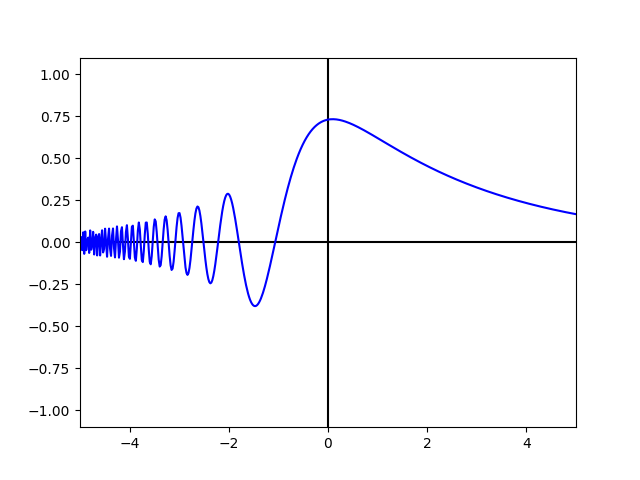
\includegraphics[width=.5\textwidth]{hw3_figure_1} & 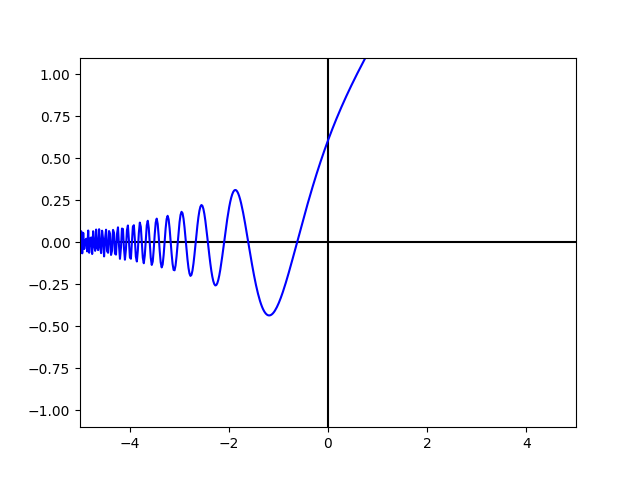
\includegraphics[width=.5\textwidth]{hw3_figure_2} \\
			$C_1=1$ and $C_2=0$ & $C_1=0$ and $C_2=1$ \\
			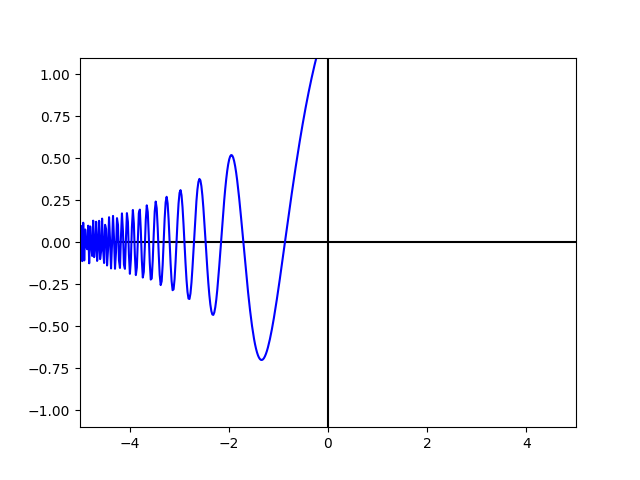
\includegraphics[width=.5\textwidth]{hw3_figure_3} & 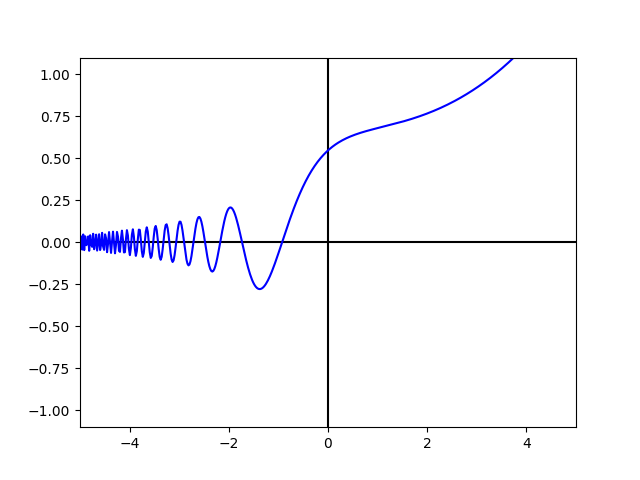
\includegraphics[width=.5\textwidth]{hw3_figure_4} \\
			$C_1=1$ and $C_2=1$ & $C_1=.5$ and $C_2=.3$ \\
		\end{tabular}
		\caption{Example solutions to equation (\ref{eq1})}
		\label{tbl:table_of_figures}
	\end{table} 
	
\problem{\#16} Show that $y-uv$ with $v(x)=e^{-\frac{1}{2}\int p(x)dx}$ and the ODE \\$y^{\prime\prime} + p(x)y^\prime + q(x)y=0$ gives the ODE $$u^{\prime\prime} + \Big[q(x) - \frac{1}{4}p(x)^2 - \frac{1}{2}p^\prime(x) \Big]u = 0$$

	Note that $v^\prime = e^{-\frac{1}{2}\int p dx} (-\frac{1}{2})p = -\frac{1}{2}pv$. Then we can derive the following
	\begin{align*}
		y^\prime & = u^\prime v + -\frac{1}{2}pvu \\
		y^{\prime\prime} & = u^{\prime\prime} v - \frac{1}{2}pvu^\prime -\frac{1}{2}p^\prime uv -\frac{1}{2}p u^\prime v - \frac{1}{4}p^2 u v\\
	\end{align*}
	Substituting into our ODE we have
	\begin{align*}
		u^{\prime\prime} v - \frac{1}{2}pvu^\prime -\frac{1}{2}p^\prime uv -\frac{1}{2}p u^\prime v + \frac{1}{4}p^2 u v + p(u^\prime v + -\frac{1}{2}pvu) + quv & = 0 \\
		v \Big(u^{\prime\prime} - \frac{1}{2}pu^\prime -\frac{1}{2}p^\prime u -\frac{1}{2}p u^\prime + \frac{1}{4}p^2 u + p(u^\prime + -\frac{1}{2}pu) + qu \Big) & = 0 \\
		v \Big(u^{\prime\prime} -\frac{1}{2}p^\prime u - p u^\prime + \frac{1}{4}p^2 u + pu^\prime + -\frac{1}{2}p^2u) + qu \Big) & = 0 \\
		v \Big(u^{\prime\prime} -\frac{1}{2}p^\prime u - \frac{1}{4}p^2 u + qu \Big) & = 0 \\
		v \Big(u^{\prime\prime} + \Big[ q  - \frac{1}{4}p^2 - \frac{1}{2}p^\prime \Big]u \Big) & = 0
	\end{align*}
	Since $v(x)=e^{-\frac{1}{2}\int p(x)dx} \neq 0$ we arrive at our desired ODE
	$$
	u^{\prime\prime} + \Big[ q  - \frac{1}{4}p^2 - \frac{1}{2}p^\prime \Big]u = 0
	$$
	
\problem{\#17} Show that for Bessel's equation, the substitution in problem 16 is $y=ux^{-1/2}$ and gives $$x^2u^{\prime\prime} + (x^2 + \frac{1}{4} - v^2)u=0$$

	Consider Bessel's equation $x^2y^{\prime\prime} + xy^\prime + (x^2-v^2)y = 0$. Dividing by $x^2$ we can put this in the form of the ODE in problem 16
	$$
	y^{\prime\prime} + x^{-1}y^\prime + \Big(1-\frac{v^2}{x^2} \Big)y = 0
	$$
	Let $q(x) = 1-\frac{v^2}{x^2}$ and $p(x) = x^{-1}$. Then let
	\begin{align*}
		\xi(x) = e^{-\frac{1}{2}\int p(x)dx} & = e^{-\frac{1}{2}\int x^{-1}dx} \\
		& = e^{-\frac{1}{2}ln(x)} \\
		& = e^{ln(x^{-\frac{1}{2}})} \\
		& = x^{-\frac{1}{2}}
	\end{align*}
	Note also that
	\begin{align*}
		p(x)^2 & = x^{-2} \\
		p^\prime(x) & = -x^{-2}
	\end{align*}
	Letting $y = u\xi$ we can substitute into our ODE as in problem 16 to obtain
	\begin{align*}
		u^{\prime\prime} + \Big[ q  - \frac{1}{4}p^2 - \frac{1}{2}p^\prime \Big]u  & = 0 \\
		u^{\prime\prime} + \Big[ \Big(1-\frac{v^2}{x^2} \Big)  - \frac{1}{4}x^{-2} + \frac{1}{2}x^{-2} \Big]u  & = 0 \\
		u^{\prime\prime} + \Big[ \Big(1-\frac{v^2}{x^2} \Big)  + \frac{1}{4}x^{-2} \Big]u  & = 0 \\
		x^2u^{\prime\prime} + \Big(x^2-v^2 + \frac{1}{4} \Big)u  & = 0 \\
	\end{align*}
	
\problem{\#20}Derive Bessel's Equation from the 4 properties in equation (21) from the text.
	
	We would like to derive Bessel's equation (alternate form) 
	$$
	y^{\prime\prime} + x^{-1}y^\prime + \Big(1-\big(\tfrac{v}{x}\big)^2\Big) y = 0
	$$
	using the properties
	\begin{align}
		\Big[x^vJ_v(x)\Big]^\prime & = x^vJ_{v-1}(x) \tag{a}\\
		\Big[x^{-v}J_{-v}(x)\Big]^\prime & = -x^{-v}J_{v+1}(x)	\tag{b} \\
		\tfrac{2v}{x}J_v & = J_	{v-1} + J_	{v+1} \tag{c} \\
		2J_v^\prime & = J_{v-1} - J_{v+1} \tag{d}
	\end{align}
	From (a) we can derive $J_v^{\prime\prime}$ as follows
	\begin{align*}
		J_v^{\prime\prime} & = \tfrac{1}{2}\big(J_{v-1} - J_{v+1}\big)^\prime \\
		J_v^{\prime\prime} & = \tfrac{1}{2} J_{v-1}^\prime - \tfrac{1}{2} J_{v+1}^\prime \\
		& = \tfrac{1}{2} \tfrac{1}{2}\big(J_{v-2} - J_{v}\big) - \tfrac{1}{2} \tfrac{1}{2}\big(J_{v} - J_{v+2}\big) \\
		& = \tfrac{1}{4} \big(J_{v-2} - 2J_v + J_{v+2}\big)
	\end{align*}
	For the second term in Bessel's equation we simplify as follows
	\begin{align*}
		x^{-1}J_v & = \tfrac{1}{2x} (J_{v-1} - J_{v+1}) \\
		& = \tfrac{1}{4v} \tfrac{2v}{x}(J_{v-1} - J_{v+1}) \\
		& = \tfrac{1}{4v} (J_{v-2} + J_v -J_v - J_{v+2}) \\
		& = \tfrac{1}{4v} (J_{v-2} - J_{v+2})
	\end{align*}
	
	The last term can be simplified as follows
	\begin{align*}
		-(\tfrac{v}{x} )^2J_v & = - \tfrac{1}{4} (\tfrac{2v}{x} )^2J_v \\
		& = - \tfrac{1}{4} (\tfrac{2v}{x})(J_{v-1} + J_v{v+1}) \\
		& = - \tfrac{1}{4} (J_{v-2} + J_{v} + J_{v} + J_v{v+2}) \\
		& = - \tfrac{1}{4} (J_{v-2} + 2J_{v}+ J_{v+2})
	\end{align*}
	
	Finally we are ready to simplify Bessel's equation
	\begin{align*}
		y^{\prime\prime} & + x^{-1}y^\prime + \Big(1-\big(\tfrac{v}{x}\big)^2\Big) y = \\
		& = \tfrac{1}{4} \big(J_{v-2} - 2J_v + J_{v+2}\big) + \tfrac{1}{4v} (J_{v-2} - J_{v+2}) + J_v - \tfrac{1}{4} (J_{v-2} + 2J_{v}+ J_{v+2}) \\
		& = \tfrac{1}{4}(-4J_{v-2}) + J_v + \tfrac{1}{4v} (J_{v-2} - J_{v+2}) \\
		& = \tfrac{1}{4v} (J_{v-2} - J_{v+2})
	\end{align*}
	
	However, a few calculations easily show this is not identically zero. There must an error somewhere.
	
	\bigbreak
	\textbf{not finished}

\large{\textbf{Section 5.4}}\\
\problem{\#4} Find a general solution to $\frac{d^2y}{dx^2} + xy = 0$ in terms of $J_v$ and $Y_v$. Indicate whether you could also use $J_{-v}$ instead of $Y_v$. Use the substitutions \\$y = ux^{1/2}, \frac{2}{3}x^{3/2}=z$. \bigbreak

	From $y = ux^{1/2}$, we obtain the following substitutions
	\begin{align*}
		\frac{dy}{dx} & = x^{\frac{1}{2}}\frac{du}{dx} + \tfrac{1}{2}x^{-\frac{1}{2}}u \\
		\frac{d^2y}{dx^2} & = x^{\frac{1}{2}}\frac{d^2u}{dx^2} + \tfrac{1}{2}x^{-\frac{1}{2}}\frac{du}{dx} - \tfrac{1}{4}x^{-\frac{3}{2}}u + \tfrac{1}{2}x^{-\frac{1}{2}}\frac{du}{dx} \\
		& = x^{\frac{1}{2}}\frac{d^2u}{dx^2} + x^{-\frac{1}{2}}\frac{du}{dx} - \tfrac{1}{4}x^{-\frac{3}{2}}u
	\end{align*}
	Substituting into $\frac{d^2y}{dx^2} + xy =  0$ we obtain
	\begin{align}
		x^{\frac{1}{2}}\frac{d^2u}{dx^2} + x^{-\frac{1}{2}}\frac{du}{dx} - \tfrac{1}{4}x^{-\frac{3}{2}}u + xux^{1/2} & =  0 \nonumber \\
		x^{\frac{1}{2}}\frac{d^2u}{dx^2} + x^{-\frac{1}{2}}\frac{du}{dx} - \tfrac{1}{4}x^{-\frac{3}{2}}u + ux^{3/2} & =  0 \nonumber \\
		x^2\frac{d^2u}{dx^2} + x\frac{du}{dx} - \tfrac{1}{4}u + ux^3 & =  0 \nonumber  \\
		x^2\frac{d^2u}{dx^2} + x\frac{du}{dx} + \big(x^3 - \tfrac{1}{4}\big)u & = 0 \label{p4eq1}
	\end{align}
	From $\frac{2}{3}x^{3/2}=z$ we obtain the following equations
	\begin{align}
		x^\frac{3}{2} = & \tfrac{3}{2}z  &  \frac{dz}{dx} & = x^\frac{1}{2}   \nonumber \\
		x^3 = & \big(\tfrac{3}{2}\big)^2z^2  & \frac{d^2z}{dx^2} & = \tfrac{1}{2}x^{-\frac{1}{2}}  \nonumber \\
		\frac{du}{dx} & = x^\frac{1}{2}\frac{du}{dz}  &  \frac{d^2u}{dx^2} & = \tfrac{1}{2}x^{-\frac{1}{2}}\frac{du}{dz} + x\frac{d^2u}{dz^2} \nonumber
	\end{align}
	Substituting these into (\ref{p4eq1}) we obtain
	\begin{align}
		x^2\frac{d^2u}{dx^2} + x\frac{du}{dx} + \big(x^3 - \tfrac{1}{4}\big)u & = 0 \nonumber \\
		x^2\Big( \frac{1}{2}x^{-\frac{1}{2}}\frac{du}{dz} + x\frac{d^2u}{dz^2} \Big) + x \Big( x^\frac{1}{2}\frac{du}{dz} \Big) + \big(x^3 - \tfrac{1}{4}\big)u & =  0 \nonumber  \\
		\tfrac{1}{2}x^{\frac{3}{2}}\frac{du}{dz} + x^3\frac{d^2u}{dz^2} + x^\frac{3}{2}\frac{du}{dz} + \big(x^3 - \tfrac{1}{4}\big)u & =  0 \nonumber  \\
		x^3\frac{d^2u}{dz^2} + \frac{3}{2}x^{\frac{3}{2}}\frac{du}{dz} + \big(x^3 - \tfrac{1}{4}\big)u & =  0 \nonumber  \\
		\big(\tfrac{3}{2}\big)^2z^2\frac{d^2u}{dz^2} + \tfrac{3}{2}\tfrac{3}{2}z\frac{du}{dz} + \Big(\big(\tfrac{3}{2}\big)^2z^2 - \tfrac{1}{4}\Big)u & =  0 \nonumber  \\
		z^2\frac{d^2u}{dz^2} + z\frac{du}{dz} + \big(z^2 - \tfrac{1}{9}\big)u & =  0 \label{p4eq2}
	\end{align}
	This is Bessel's Equation with $v=\frac{1}{3} \notin \mathbb{Z}$. Thus $u= C_1J_{1/3}(z) + C_2J_{-1/3}(z)$ is a general solution to (\ref{p4eq2}). Subtituting we obtain a general solution to our original ODE
	$$
	y= x^{-\frac{1}{2}} \Bigg[ J_{1/3} C_1 \Big(\tfrac{2}{3}x^{3/2}\Big) + C_2 J_{-1/3}\Big(\tfrac{2}{3}x^{3/2}\Big) \Bigg]
	$$
	

\end{document}
